\documentclass{article}

\newcommand{\code}[1]{\texttt{#1}}
\usepackage[margin=1in]{geometry}
\usepackage[final,formats]{listings}
\usepackage{float}
\usepackage{hyperref}
\usepackage{graphicx}

\lstnewenvironment{tsllisting}[1][]
{\lstset{
    escapeinside={(*@}{@*)},
    basicstyle=\footnotesize\ttfamily,
    keywordstyle=\bfseries,
    keywordstyle=\bfseries,
    sensitive=false,
    morekeywords={template, endtemplate, process, controllable, forever, wait, return, assert, goal, instance},
    identifierstyle=, 
    commentstyle=\slshape, 
    stringstyle=, showstringspaces=false,
    sensitive=false,
    morecomment=[s]{/*}{*/},
    numberstyle=\tiny,
    stepnumber=1,
    numbersep=1pt,
    emphstyle=\bfseries,
    belowskip=0pt,
    aboveskip=0pt,
    #1
}}{}

\begin{document}

\title{Termite Tutorial}
\author{Adam Walker \and Leonid Ryzhyk}

\maketitle

\tableofcontents

\section{Introduction}

Before reading this tutorial, it is recommended that you read \cite{Ryzhyk_WKLRSV_14} to understand the main concepts of the Termite tool. Additionally, the reader is referred to \cite{Walker_Ryzhyk_14} to further understand the driver synthesis algorithm.

In this tutorial we will generate a driver for a hypothetical one bit GPIO device. The operating system may request that the driver set and clear the bit. The device exposes a simple interface consisting of a single 8 bit register. One of these bits is connected to the external GPIO output; the rest are ignored. The driver that will be automatically synthesized writes the appropriate value to this register to fulfill the OS request. 

The thoroughly commented source code of this example is available in the \code{documentation/GPIO} directory in the Termite repository at \url{http://github.com/termite2/Termite}.

\section{Specifications}

The inputs to the Termite specification tool are:
\begin{enumerate}
    \item the device specification
    \item the operating system specification
    \item the empty driver template
    \item the class specification that declares the interfaces of the above 3 components
    \item the main file that connects everything together
\end{enumerate}

We will describe each of these in turn.

\subsection{Device specification}

The device we are specifying is a simple 1 bit GPIO device whos output bit can be accessed by writing to a register. We declare a 1 bit variable named output to keep track of the current state of the GPIO output. The GPIO device has two interface methods - \code{get\_value()} for querying the current state of the GPIO pin, which will be used by the OS specification later, and \code{write8} which the driver can use to write to the register connected to the GPIO pin. 

\code{get\_value()} operates as expected - it simply returns the value that is currently being output. Note that \code{get\_value} is a virtual function, it does not correspond to any run time behavior and is only used by the OS specification to enforce correct behavior. 

\code{write8} sets the GPIO output to bit 0 of the value written, and, it additionally notifies the OS that the value was set using \code{os.value\_set()}. This is also a virtual function. As we will see later, this is used to prevent the driver from changing the value of the GPIO when it was not requested to.

\begin{figure}[H]
\lstset{numbers=left}
\begin{tsllisting}
import <class.tsl>

template gpio_dev_inst(gpio_os os)

derive gpio_dev;

uint<1> output;

task controllable void write8(uint<8> val){
    output = val[0:0];
    os.value_set(output);
};

function uint<1> get_value(){
    return output;
};

endtemplate
\end{tsllisting}
\end{figure}

\subsection{OS specification}

In this example, the operating system specification is the most complex specification. Unlike the device, the OS contains an active process. The role of this process is to generate driver requests, dispatch them, and ensure that the driver completed its job. It is similar to a test harness for the driver. 

The process \code{pos} loops forever (the \code{forever} block), nondeterministically choosing one of two driver requests to make. The forever block must contain a \code{pause} statement to that its body cannot complete instantaneously. The \code{choice} block non-deterministically decides to either set or clear the GPIO bit. We will only consider the \code{set\_bit()} function as \code{clr\_bit()} is very similar. 

The \code{set\_bit} task ensures that the \code{making\_request} flag is \code{true} whenever execution is in the driver function. This is to ensure that the driver does not make changes to the GPIO bit when not requested to as explained below. It then calls the driver method and checks that the driver performed the required action by calling the device's \code{get\_value()} function and checking that it is the expected value.

All that remains is the \code{value\_set()} virtual callback function. This is called by the device whenever the value of the GPIO pin is changed. It asserts that we are currently making a request using the \code{making\_request} flag. This prevents the driver from changing the GPIO output when not requested to. It does not, however, prevent the driver from changing the value to a temporarily wrong value during the driver call. Handling this case is covered in section \ref{sec:extending}.

\begin{figure}[H]
\lstset{numbers=left}
\begin{tsllisting}
import <class.tsl>

template gpio_os_inst(gpio_drv drv, gpio_dev dev)

derive gpio_os;

process pos {
    forever{
        choice{       
            set_bit();
            clr_bit();
            {};      
        };
        pause;      
    };
};

bool making_request = false;

task void set_bit(){
    making_request = true;
    drv.set_bit(); // call the driver
    making_request = false;

    assert(dev.get_value() == 1'h1);
};

task void clr_bit(){
    making_request = true;
    drv.clr_bit(); // call the driver
    making_request = false;

    assert(dev.get_value() == 1'h0);
};

procedure void value_set(uint<1> value){
    // Only allow the GPIO pin to change its state when there is a request in progress
    assert(making_request);
};

endtemplate
\end{tsllisting}
\end{figure}

\subsection{Driver template}

The driver template is what the Termite tool will interactively fill in to create the final driver. The driver consists of two methods: \code{set\_bit()} and \code{clr\_bit()} as declared in the class specification. They neither return a result or take any arguments. You will notice that the body of each driver method contains only an ellipsis. This is referred to as a magic block. It is Termite's job to replace all magic blocks with driver code. When we run the tool in section \ref{sec:running} we will interactively ask Termite to fill these in.

\begin{figure}[H]
\lstset{numbers=left}
\begin{tsllisting}
import <class.tsl>
import <gpio.tsl>

template gpio_drv_inst(gpio_dev_inst dev, gpio_os os)

derive gpio_drv;

task uncontrollable void set_bit(){
    ...;
};

task uncontrollable void clr_bit(){
    ...;
};

endtemplate
\end{tsllisting}
\end{figure}

\subsection{Class specification}

The class specification declares three abstract interfaces, one each for the driver, device and operating system components. 

\begin{figure}[H]
\lstset{numbers=left}
\begin{tsllisting}
template gpio_drv

task uncontrollable void set_bit();
task uncontrollable void clr_bit();

endtemplate

template gpio_dev

function uint<1> get_value();

endtemplate

template gpio_os

procedure void value_set(uint<1> value);

endtemplate
\end{tsllisting}
\end{figure}
\subsection{Main file}

The main file simply creates an instance of each of the components described earlier and ties them together.

\begin{figure}[H]
\lstset{numbers=left}
\begin{tsllisting}
import <os.tsl>
import <gpio.tsl>
import <drv.tsl>

template main

instance gpio_os_inst  os  (drv, dev);
instance gpio_dev_inst dev (os);
instance gpio_drv_inst drv (dev, os);

endtemplate
\end{tsllisting}
\end{figure}

\section{Running the tool}
\label{sec:running}

Enter the directory of the specifications and run the tool with:

\[\code{termite -i main.tsl -s}\]

\code{-i} specifies the input file and \code{-s} tells Termite to perform synthesis.

It should only take a few seconds to synthesize and then launch a graphical debugging console. We will now ask Termite to fill in the magic blocks. 

\section{Generating the driver}

Once the graphical debugger has been launched, switch to the \code{drv.tsl} tab in the rightmost pane. The window should look like figure \ref{fig:screenshot_before}. Notice the yellow highlighted magic blocks. We are now going to generate the code that goes in these magic blocks. Click on the first magic block and then click on the button with the gears icon at the top of the page. A line of code should be automatically generated above the magic block. Click the gears one more time. This time the magic block should be replaced by \code{\{\}}, indicating that there is nothing more to do in the function. 

Repeat the above steps for the second magic block. The \code{drv.tsl} file should appear as in figure \ref{fig:screenshot_after}. You should convince yourself that the generated code is correct. Congratulations, you have generated your first Termite driver!

You may save \code{drv.tsl} and then rerun Termite. As there are no magic blocks, Termite is now acting as a verifier. It should report that synthesis succeeded. 

\begin{figure}
    \center
    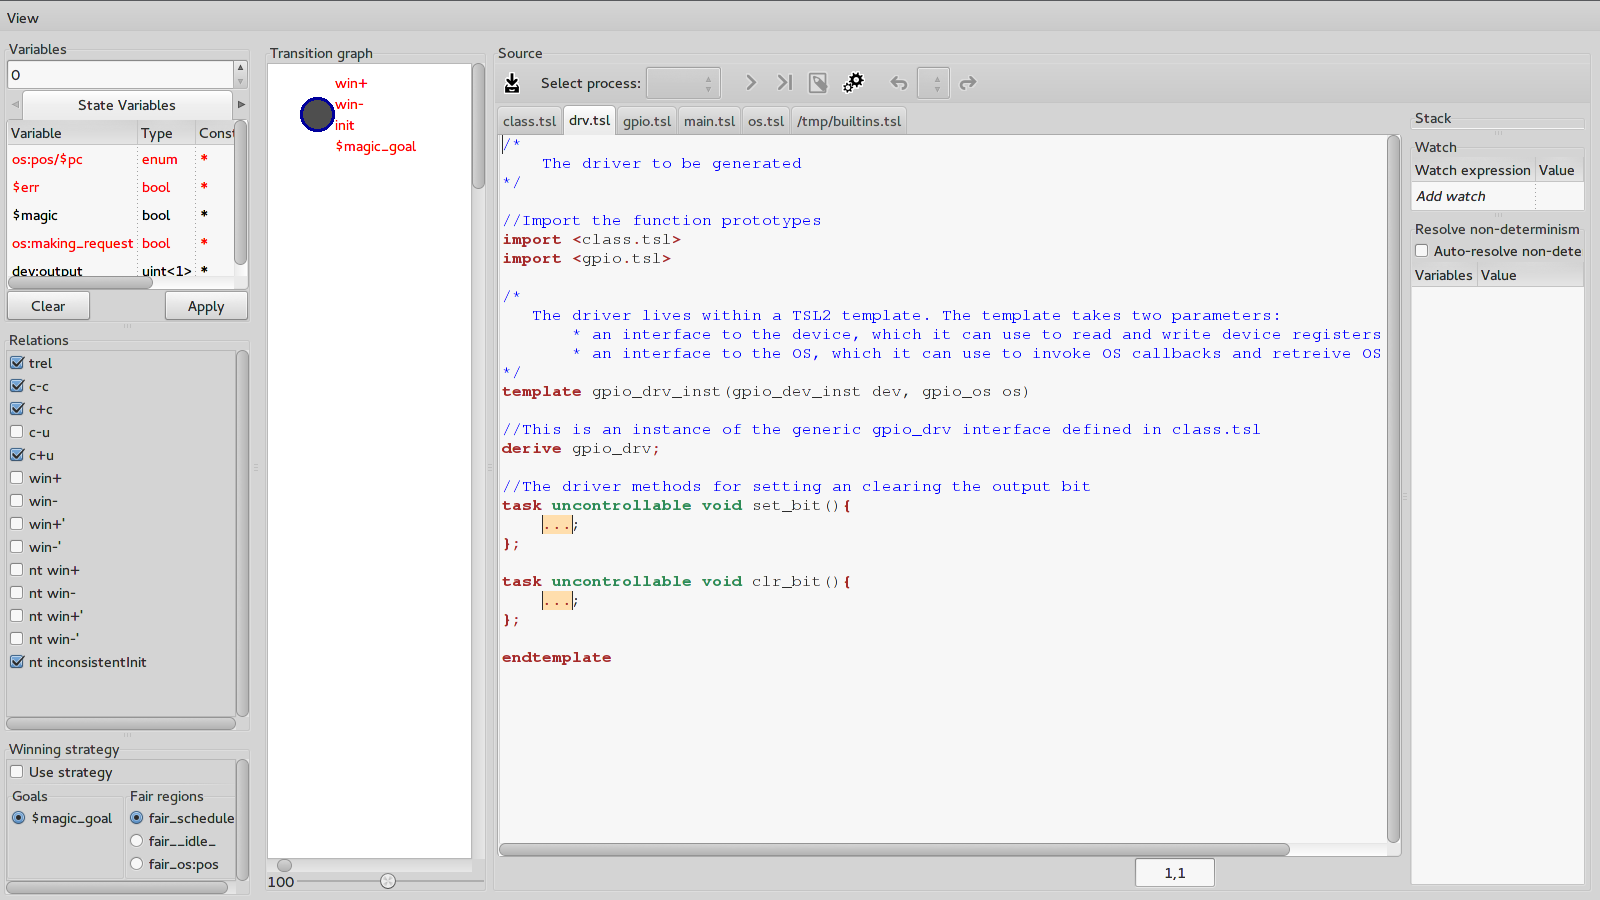
\includegraphics[width=\linewidth]{figs/debugger1.png}
    \caption{The debugger after switching to the \code{drv.tsl} tab}
    \label{fig:screenshot_before}
\end{figure}

\begin{figure}
    \center
    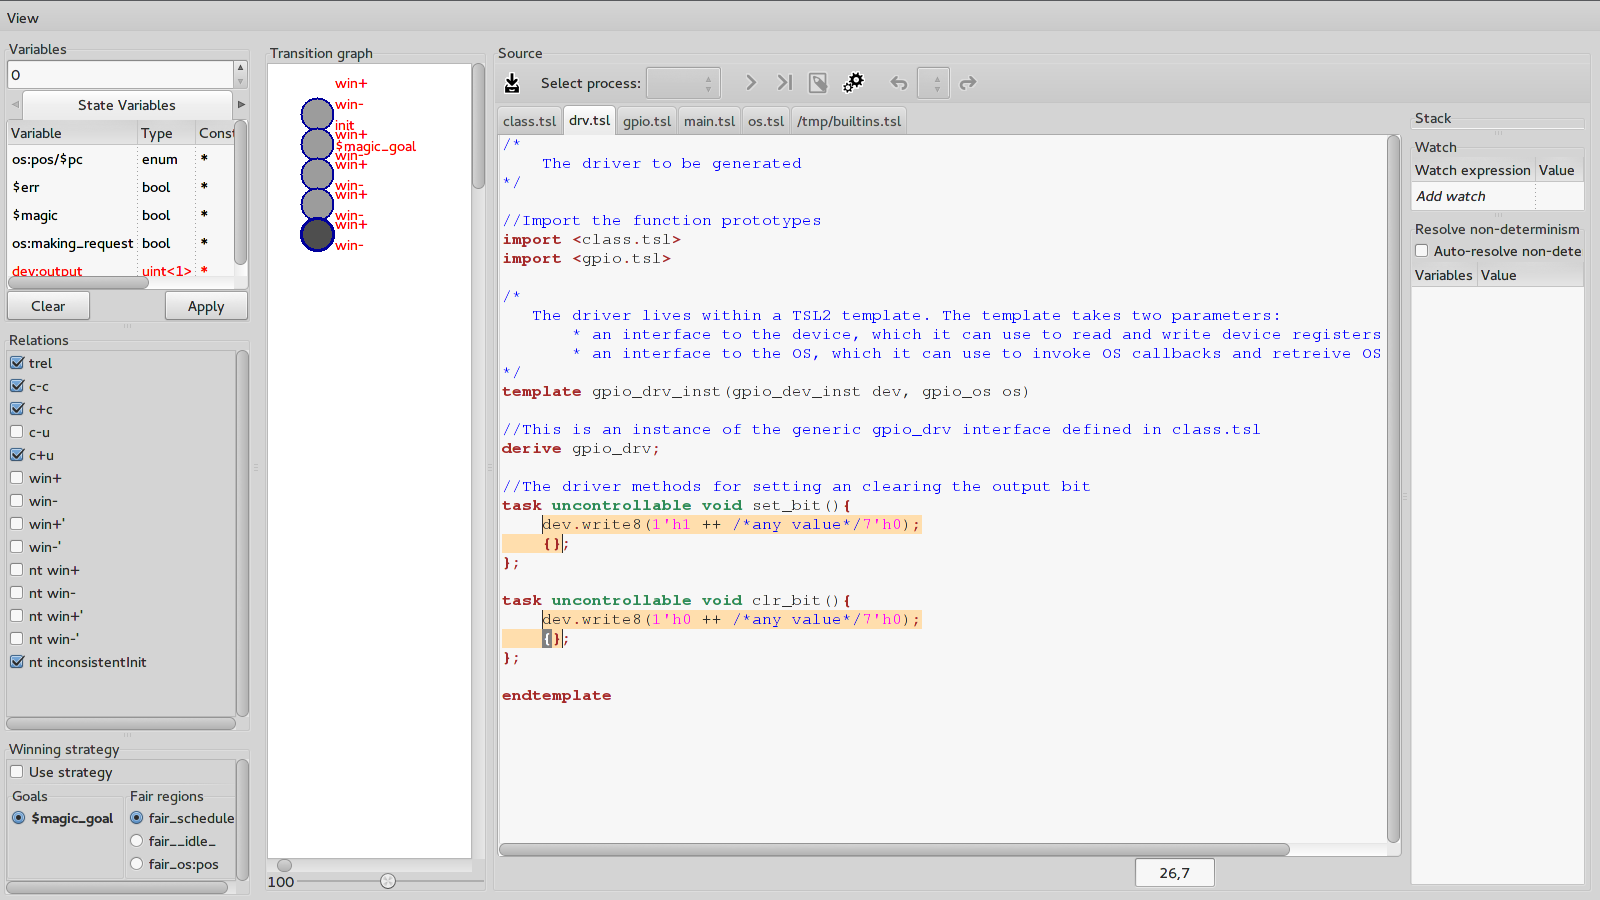
\includegraphics[width=\linewidth]{figs/debugger2.png}
    \caption{The debugger after generating code}
    \label{fig:screenshot_after}
\end{figure}

\section{Extending the specifications}
\label{sec:extending}

\section{Further reading}
An extensively commented I2C driver example is available at \url{https://github.com/termite2/Termite/tree/master/documentation/i2c}. It demonstrates more advanced usage of Termite on a real device. 

\bibliography{bib}
\bibliographystyle{abbrv} 

\end{document}
